\documentclass{article}

\usepackage{arxiv}
\usepackage[utf8]{inputenc} 
\usepackage[T1]{fontenc}    
\usepackage{hyperref}      
\usepackage{url}            
\usepackage{booktabs}       
\usepackage{amsfonts}       
\usepackage{nicefrac}       
\usepackage{microtype}      
\usepackage{cleveref}       
\usepackage{graphicx}
\usepackage{natbib}
\usepackage{doi}
\usepackage[portuguese]{babel}
\usepackage{caption}
\usepackage{braket}
\usepackage{amsmath}
\usepackage{algpseudocode}
\usepackage{algorithm}
\usepackage{mathtools}
\usepackage{titlesec}

\DeclarePairedDelimiter\floor{\lfloor}{\rfloor}

\setcounter{secnumdepth}{5}
\setcounter{tocdepth}{5}

\makeatletter
\renewcommand\subsubsubsection{\@startsection{paragraph}{4}{\z@}{-2.5ex\@plus -1ex \@minus -.25ex}{1.25ex \@plus .25ex}{\normalfont\normalsize\bfseries}}
\newcommand\subsubsubsubsection{\@startsection{subparagraph}{5}{\z@}{-2.5ex\@plus -1ex \@minus -.25ex}{1.25ex \@plus .25ex}{\normalfont\normalsize\bfseries}}
\makeatother


\title{Quantum Oracles - Como transformar problemas clássicos em quânticos}

\date{\today}



\author{ 
	\href{https://orcid.org/0009-0008-9134-5974}{
\includegraphics[scale=0.06]{orcid.pdf}\hspace{1mm}Alexandre Silva}\\
	Ciências da Computação\\
	UNIVEM - Centro Universitário Eurípides de Marília\\
	\And
	\href{http://lattes.cnpq.br/5170103189904688}{\hspace{1mm}Luis Hilário Tobler Garcia} \\
	Ciências da Computação\\
	UNIVEM - Centro Universitário Eurípides de Marília\\
	\And
	\href{http://lattes.cnpq.br/7265559606596355}{\hspace{1mm}Maúricio Duarte} \\
	Tecnologia da Informação \\
	Fatec Garça – Deputado Julio Julinho Marcondes de Moura\\
}

\graphicspath{ {../images/} }

\renewcommand{\headeright}{}
\renewcommand{\undertitle}{}
\renewcommand{\shorttitle}{}


\hypersetup{
	pdftitle={Quantum Oracles - Como transformar problemas classicos em quanticos},
	pdfsubject={quantum computing, computer science, ciências da computação, computação quântica, algoritmos, algorithms, problem solving, problems, solução de problemas, problemas},
	pdfauthor={Alexandre Silva},
	pdfkeywords={quantum oracles, quantum, quantum computing, algoritmos, algorithms, problems, problemas},
}

\begin{document}
\maketitle
\begin{abstract}
	A partir do uso de quantum Oracles e outros fatores quânticos, como a superposição, foram feitos \emph{5 mini-projetos}. O objetivo desses projetos foi tentar responder se é possível transformar certos problemas em quânticos e se realmente tal transformação vale a pena. Após os testes foi possível ver que, há casos em que a versão quântica apresenta um aproveitamento igual ou um pouco superior, contudo ainda é necessário o uso de computadores clássicos para conseguir melhores resultados.
\end{abstract}


\section{Introdução}
Hoje, não é difícil ver alguém falando sobre computadores quânticos e como essas máquinas vão mudar o nosso futuro. Contudo, muitas dessas frases acabam se levando por extrapolações e/ou usos indevidos de ficção. Neste artigo, mostrarei que nem tudo é possível ser feito com um computador quântico atual, assim como existem pequenas áreas que se beneficiam ao máximo dessa nova tecnologia.\\
Para esse feito, serão mostrados \emph{5 mini-projetos} usando o \href{https://www.ibm.com/quantum/qiskit}{qiskit}, framework open source da \href{https://www.ibm.com/}{IBM}, e os resultados obtidos após executar os algoritmos quânticos e seus relativos em computação clássica.\\
Tais mini-projetos foram os seguintes: Explorador de Arquivos \ref{file-explorer}, conversão de milhas para quilômetros \ref{conversion}, Torres de Hanoi \ref{hanoi}, Buckshot Roulette \ref{buckshot} e QRAM \ref{qram}. Todas as implementações podem ser encontradas nesse  \href{https://github.com/Dpbm/scientific-initiation-1-quantum-oracles}{repositório do GitHub}.\\
Para a criação desses projetos, foram usados os Quantum Oracles em conjunto com alguns algoritmos, explorando efeitos quânticos e algumas outras técnicas, clássicas e quânticas, para cada caso específico.

\section{Oracles}
Partindo da ideia das \emph{Oracle Turing Machines} \cite{SOARE2009368}\cite{amreen_oracle}\cite{kalyanasyndaram_2021_mod04lec23}\cite{e21080800}, os Oracles são modelos matemáticos ideais, usados para abstrair certas partes de um algoritmo principal, em formato de caixa preta, facilitando a análise do algoritmo, assim como sua descrição matemática. Tais máquinas podem ser vistas, também, como uma função, recebendo uma entrada $x$ e retornando $f(x)$ em tempo $O(1)$. Em computação clássica, esse modelo não possui implementação real, sendo usado apenas descrições formais para problemas de decisão.\\
Contudo, em computação quântica, é possível implementar esses componentes e tomar proveito de sua estrutura e efeitos quânticos para conseguir um \emph{Speed-up} em relação aos algoritmos clássicos, como mostrado pelo algoritmo de Deutsch–Jozsa \cite{Fan_2007}. Além disso, os Oracles possuem um papel importante ao demonstrar a complexidade de um circuito, alguns dos meios utilizados são: profundidade (\emph{depth}), calculando o maior caminho que uma informação percorre no circuito, ou ainda, a quantidade de gates aplicados. No entanto, essas maneiras acabam se prejudicando ao \emph{transpilar} o circuito para uma outra máquina, variando então a complexidade de acordo com a topologia e com os gates fisicamente implementados. Para solucionar isso, outra maneira de calcular é inserir partes do circuito em um Oracle, e descrever sua complexidade a partir da quantidade de vezes que ele chamado, também conhecido como \emph{query complexity} \cite{odonnell_2015_lecture} \cite{e21080800}.

\subsection{Tipos de Oracles}
A partir da definição dos Quantum Oracles, podemos classificá-los em relação a suas estruturas e maneiras de computar os dados.

\subsubsection{Phase Oracle}
O Phase Oracle, é o formato mais conhecido e usado em circuitos quânticos. Algoritmos como os de  Deutsch–Jozsa, Grover, Simon e Bernstein–Vazirani, tomam proveito desse artifício para se sobressair em relação às soluções clássicas. 

\subsubsubsection{Funcionamento Padrão}
Seu funcionamento, se baseia em atribuir uma fase global ao circuito, tomando proveito de fatores como \emph{Phase Kickback} (fase passa do target do CNOT e é aplicado no qubit de controle), para  conseguir modificar valores em superposição.

\begin{center}
	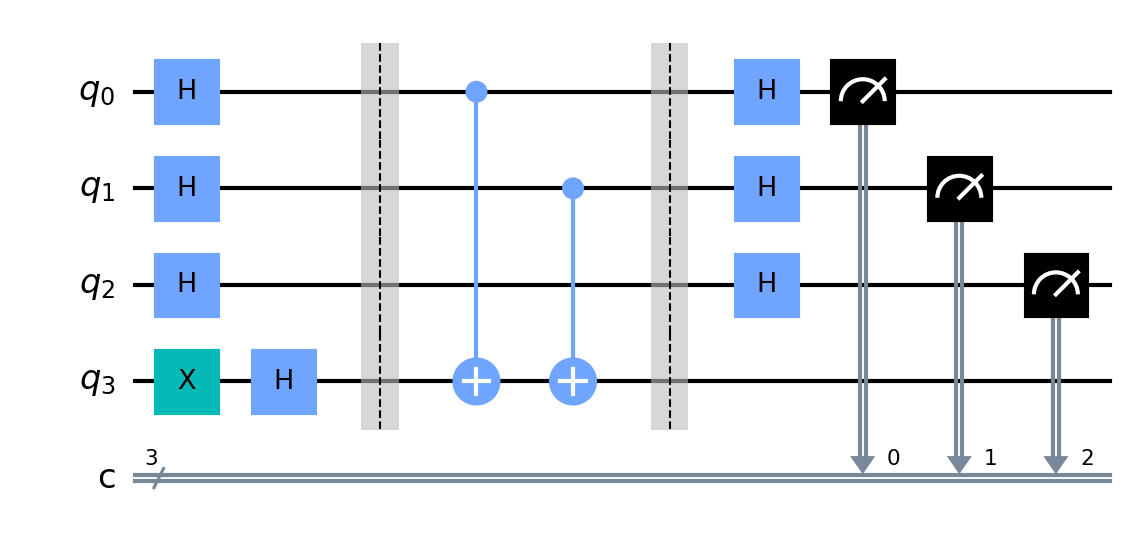
\includegraphics[scale=0.3]{phase_oracle_1.png}
	\captionof{figure}{Exemplo - Phase Oracle}
	\label{fig:phase-oracle-1}
\end{center}

Na Imagem \ref{fig:phase-oracle-1}, foi introduzida uma fase $\pi$ no qubit auxiliar ($q3$) através do estado  $\ket{-}$. Essa fase será responsável por modificar os valores na matriz unitária final. Nessa configuração, os CNOTs agem de uma forma um tanto diferente do convencional, aqui,  ao invés de apenas inverter o valor do qubit no target quando o qubit de controle for $1$, devido a fase, ele também agirá como um gate $Z$ sendo aplicado no estado do qubit de controle. Sendo assim, ao aplicar $CNOT\ket{-}\ket{+}$ (qubit menos significativo à direita), o estado se torna ${\frac{1}{\sqrt{2}}}{(\ket{0}\ket{-} - \ket{1}\ket{-})}$, e ao remover a superposição com o $H$, a saída se torna: ${\frac{1}{\sqrt{2}}}{(\ket{+}\ket{1} - \ket{-}\ket{1})}$. Dessa forma, o qubit que antes estava como controle do gate, sofre a ação do \emph{Phase Kickback}, e seu estado padrão $\ket{0}$ é modificado pela fase e se torna $\ket{1}$. A partir disso, é possível encodar um certo valor binário dentro do Oracle e utilizá-lo para cálculos. 

\subsubsubsection{Versão Minimal Oracle}
Além disso, esse não é o único formato possível de Phase Oracle. Por apenas aplicar uma fase em certas bit-strings, o qubit auxiliar pode ser removido, e a fase pode ser adicionada através de gates $Z$controlados (ou outro gate capaz de aplicar uma fase $\pi$ para certa bit-string), mas ainda assim mantendo a natureza unitária, podendo ser visto também como um Minimal Oracle.

\begin{center}
	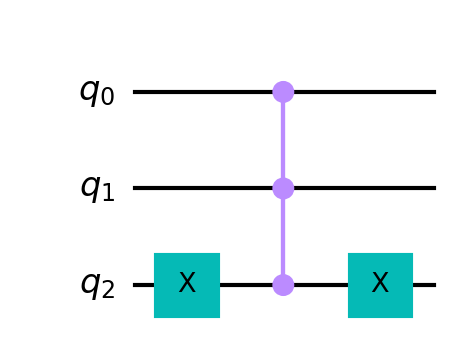
\includegraphics[scale=0.3]{phase_oracle_2.png}
	\captionof{figure}{Exemplo Phase Oracle como um Minimal Oracle}
	\label{fig:phase-oracle-2}
\end{center}

No exemplo da imagem \ref{fig:phase-oracle-2}, foi adicionado um gate $MCP$ com a fase global $\pi$ e dois gates $X$ para inverter os qubits queremos que tenham o valor $0$, codificando assim o valor $011_{2}$ ou $3_{10}$.

\begin{center}
	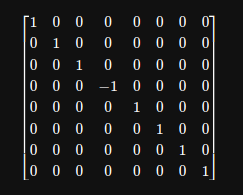
\includegraphics[scale=0.5]{phase_oracle_unitary.png}
	\captionof{figure}{Matriz unitária do Phase Oracle da imagem \ref{fig:phase-oracle-2}}
	\label{fig:phase-oracle-unitary}
\end{center}

Assim, é possível verificar que ao criar esse circuito, é mantida a matriz identidade mas com a fase ($-1$) no valor $1$ na coluna relativa à $011_{2}$ (figura \ref{fig:phase-oracle-unitary}). 


\subsubsection{Boolean Oracle}
O Boolean Oracle, por sua vez, apresenta um funcionamento semelhante ao do Phase Oracle. Contudo, neste não é provida uma fase. Dessa forma, o Oracle age como uma função Booleana convencional, mapeando as entradas para valores de saída.

\begin{center}
	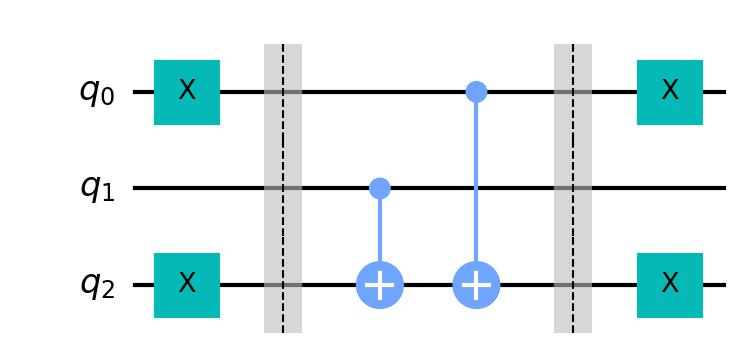
\includegraphics[scale=0.3]{balanced-oracle.png}
	\captionof{figure}{Exemplo de Oracle Booleano}
	\label{fig:boolean-oracle}
\end{center}

O Oracle implementado na figura \ref{fig:boolean-oracle}, pode ser reutilizado para o algoritmo de Deutsch-Jozsa, bastando apenas introduzir uma fase, e o Boolean Oracle se comportará como um Phase Oracle.

\subsubsection{Minimal Oracle}
Como já citado anteriormente, o Minimal Oracle possui uma função que, em sua essência, é unitária, não requerendo qubits adicionais. Sendo assim, este pode ser tanto Booleano como um Phase Oracle, dependendo de sua implementação.

\begin{center}
	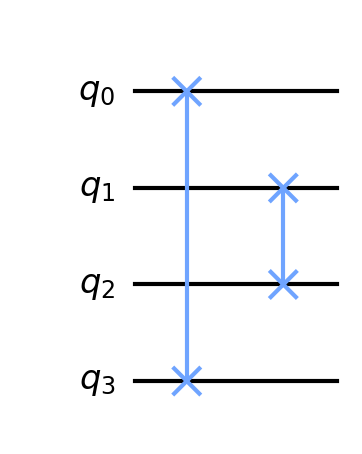
\includegraphics[scale=0.3]{minimal-oracle.png}
	\captionof{figure}{Exemplo de Minimal Oracle}
	\label{fig:minimal-oracle}
\end{center}

No exemplo da figura \ref{fig:minimal-oracle}, foram utilizados dois $SWAP$ para inverter a ordem dos valores. Com isso, a matriz final ainda se mantém unitária, com apenas valores invertidos em certas posições.

\subsubsection{QFT(Quantum Fourier Transform)}
O QFT, em suma, é um algoritmo quântico usado para pegar o período de um estado e projeta-lo na base $X$ (ou também conhecido como base de Fourier). Esse algoritmo, toma como base a transformada discreta de Fourier e aplica essa transformação em estados quânticos.\\
Mesmo sendo um algoritmo por si só, sua aplicação em circuitos se dá seguindo o formato de Oracles.

\begin{center}
	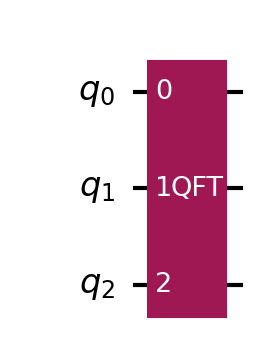
\includegraphics[scale=0.3]{QFT_1.png}
	\captionof{figure}{Exemplo do Oracle de QFT}
	\label{fig:QFT}
\end{center}

\begin{center}
	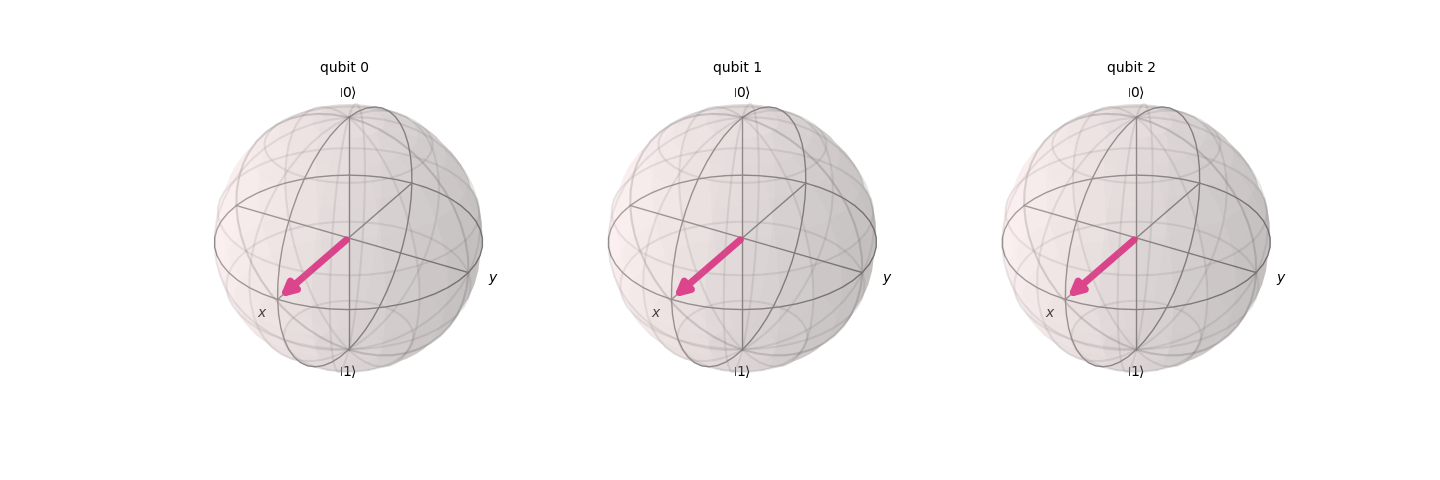
\includegraphics[scale=0.3]{QFT_1_bloch.png}
	\captionof{figure}{Valores mapeados na base de Fourier}
	\label{fig:QFT-bloch}
\end{center}


\subsubsection{Outros Oracles}
Além dos Oracles citados, é possível encontrar na literatura citações descrevendo o Oracle de Simon, o de Deutsch-Jozsa, etc. No entanto, esses são implementações de Oracles já mostrados e além disso, para o desenvolvimento deste projeto, os Oracles mais relevantes são o Phase e Boolean. Portanto, não há a necessidade de profundas investigações dessas subcategorias de Oracles.


\section{Desenvolvimento}

\subsection{Explorador de Arquivos} \label{file-explorer}

Imagine um computador quântico, com um sistema operacional quântico, capaz de interagir não apenas com a parte quântica, mas também com uma porção clássica a qualquer momento que for necessário. Essa máquina, possui todas as capacidades de um computador pessoal mais as capacidades de um computador quântico atual.\\
Pensando nas partes desse sistema, como seria possível pegar arquivos da memória?\\
Com essa ideia, foram testados alguns modelos de implementação de um circuito para essa finalidade.

\subsubsection{Algoritmos usados}

\subsubsubsection{Grover}
O algoritmo evidente para esse problema é o algoritmo de Grover. Este realiza buscas em "bancos de dados" (bit strings) desorganizados em tempo $O(\sqrt{2^n})$, do qual $n$ é o número de qubits usados. Nele, usamos um circuito do qual amplificam-se as probabilidades de encontrar os valores marcados no Oracle.

\begin{center}
	\includegraphics[scale=0.3]{Grover.png}
	\captionof{figure}{Exemplo algoritmo de Grover com $3$ qubits}
	\label{fig:grover-default-circuit}
\end{center}

Para esse circuito, é preciso adicionar o conjunto $Oracle + Diffuser$ $k$ vezes, sendo $k \approx { {\pi \over {4 \sqrt{a\over{2^n}}}} - {1\over2}  }$, do qual $a$ representa o número de valores marcados pelo Oracle. Como nesse projeto, visamos encontrar apenas $1$ arquivo encodado, não há necessidade de usar tal relação, sendo necessário apenas uma aplicação do conjunto para alcançar bons resultados.\\
Contudo, mesmo sendo o melhor algoritmo, conhecido, para buscas em computação quântica, foi testado também hipóteses para possíveis maneiras de melhor os valores das distribuições finais. Para isso, foram testadas inúmeras combinações de rotações $RY$ e foram comparadas com o convencional usado pelo algoritmo ($H$).

\begin{center}
	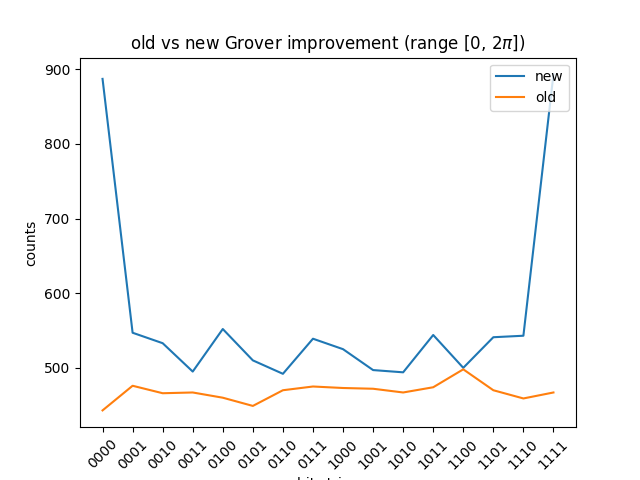
\includegraphics[scale=0.5]{improvement-grover-algorithm-4bits-0-to-2pi.png}
	\captionof{figure}{Comparação usando o algoritmo de Grover convencional e o algoritmo modificado com o melhor ângulo (entre $[0, 2\pi]$) para cada bit-string de quatro bits}
	\label{fig:best-angle-grover}
\end{center}

Ao utilizar as rotações específicas para cada bit-string, é possível conseguir melhores resultados ao medir os valores na saída, se sobressaindo em relação a rotação padrão.

\begin{center}
	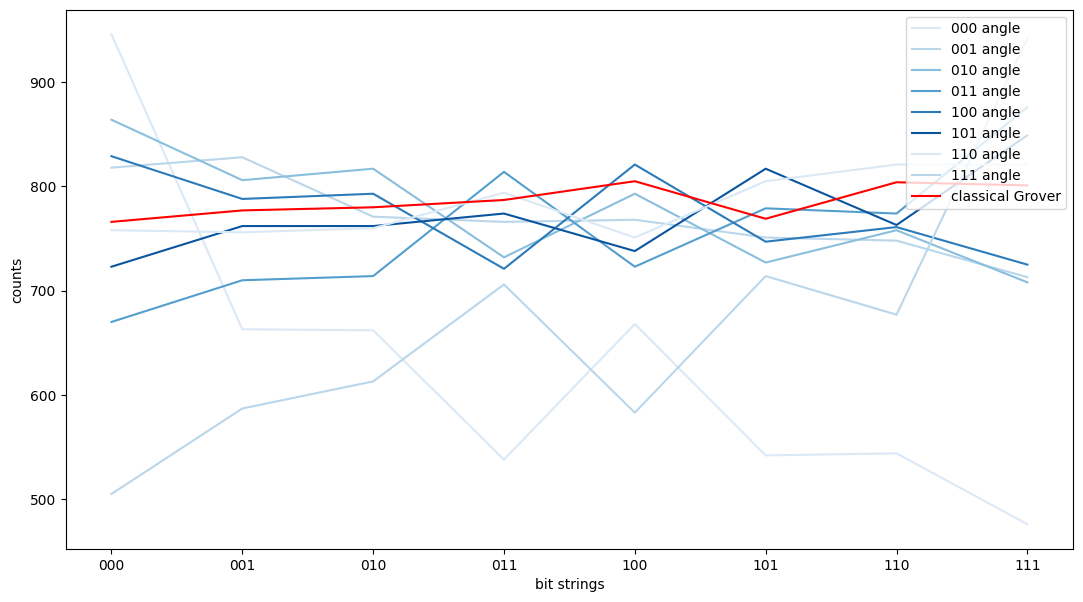
\includegraphics[scale=0.4]{new-grover-test-different-bit-strings-with-optimal-angles.png}
	\captionof{figure}{Teste utilizando os melhores ângulos de cada bit-string em bit-strings diferentes}
	\label{fig:best-angles-diff-bit-strings-grover}
\end{center}

No entanto, ao utilizar esses valores com outras bit-strings, os resultados não conseguem alcançar tal limiar, além modificar as outras probabilidades de forma irregular. Sendo assim, a rotação convencional é a melhor na maioria das vezes.\\
Além disso, para bit-strings de dois bits, utilizar a superposição dada por $H$ se mostra a melhor alternativa.

\begin{center}
	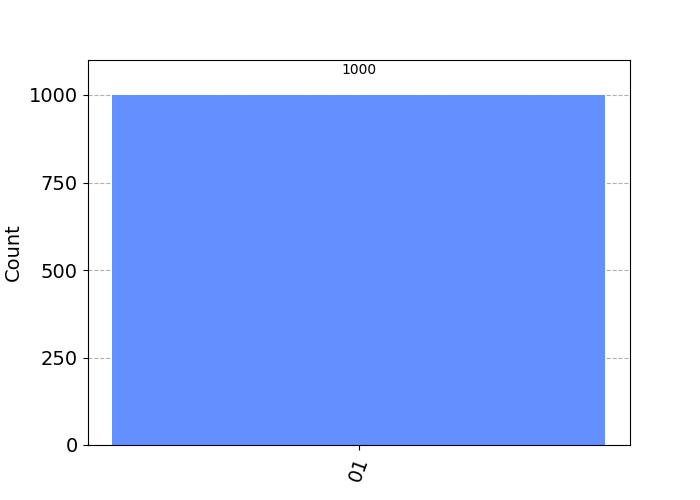
\includegraphics[scale=0.5]{classical_grover_for_1_bit_strings_l2_outcomes.png}
	\captionof{figure}{Resultado Grover padrão encodado uma bit-string de 2 bits}
	\label{fig:l2-grover-classical-outcomes}
\end{center}

\begin{center}
	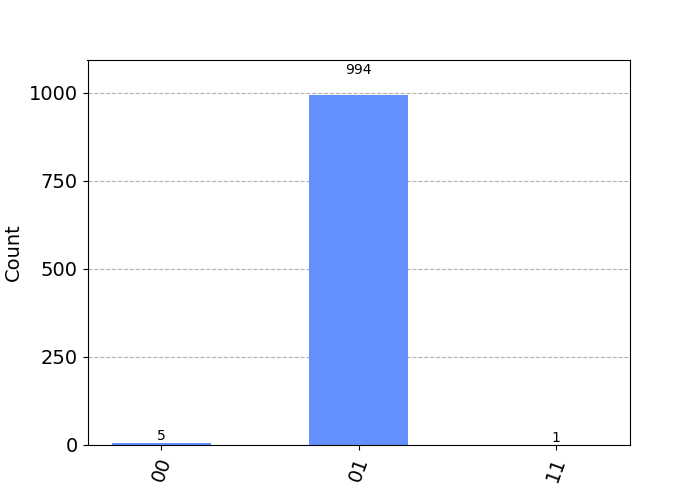
\includegraphics[scale=0.5]{new_grover_for_1_bit_strings_l2_outcomes.png}
	\captionof{figure}{Resultado Grover modificado encodado uma bit-string de 2 bits}
	\label{fig:l2-grover-new-outcomes}
\end{center}

Com isso, para ter o melhor dos dois mundos, foi usado uma versão híbrida do algoritmo. Assim, para criar o circuito, é passado o valor a ser encodado por uma Hash-Table com os ângulos otimizados. Dessa forma, é possível maximizar as probabilidades de encontrar, nesse caso, o arquivo que está sendo procurado.

\subsubsubsection{Diferença de conjuntos}
Sobrepondo dois Phase Oracles distintos, com ranges de valores diferentes, é realizada a operação de diferença entre conjuntos \cite{sanchezrivero2023initial}.

\begin{center}
	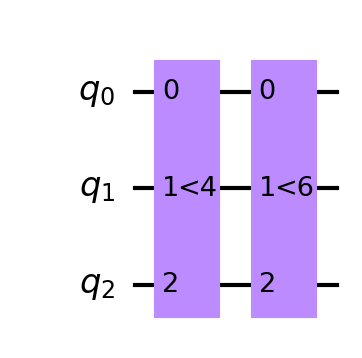
\includegraphics[scale=0.3]{less_than.png}
	\captionof{figure}{Exemplo - diferença de conjuntos}
	\label{fig:less-than-circuit}
\end{center}

Nesse exemplo \ref{fig:less-than-circuit} foi encodado no primeiro Oracle o set $\{000, 001, 010, 0110\}$ e no segundo $\{000, 001, 010, 011, 100, 101\}$.

\begin{center}
	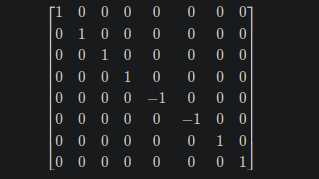
\includegraphics[scale=0.5]{less_than_unitary.png}
	\captionof{figure}{Resultado da diferença de conjuntos}
	\label{fig:less-than-circuit-unitary}
\end{center}

Ao sobrepô-los \ref{fig:less-than-circuit-unitary}, apenas os valores $\{100, 101\}$ permaneceram com a fase, representando então a sobreposição delas.


\subsubsection{Solução}

Para a solução do problema, foi criado uma hash function $C: v \to c$, da qual $v$ é o path de um arquivo e $c$ sua bit-string respectiva. Com essa função em mãos, podemos utilizar o conjunto dos valores retornados e encodá-los em um Phase Oracle, criando então uma Look-Up-Table para os arquivos existentes na máquina (agindo como a memória).\\
Além disso, é necessário utilizar um segundo Oracle para a pesquisa, encodando todos os valores existentes, menos os que foram requisitados. Assim, ao realizar a diferença entre conjuntos, apenas os valores procurados se manterão marcados.

\begin{center}
	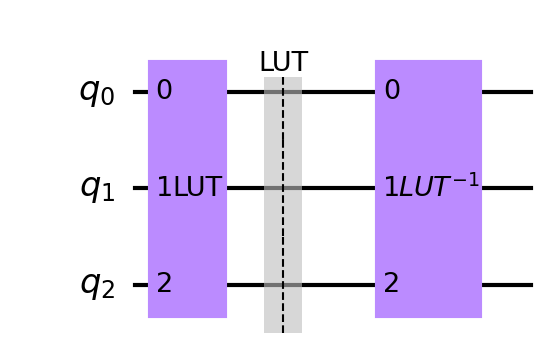
\includegraphics[scale=0.4]{sets-difference-look-up-table-oracle.png}
	\captionof{figure}{Diferença de conjuntos com as Look-Up-Tables}
	\label{fig:luts}
\end{center}


Por fim, é usado o aprimoramento dos ângulos para conseguir melhores probabilidades.

\begin{center}
	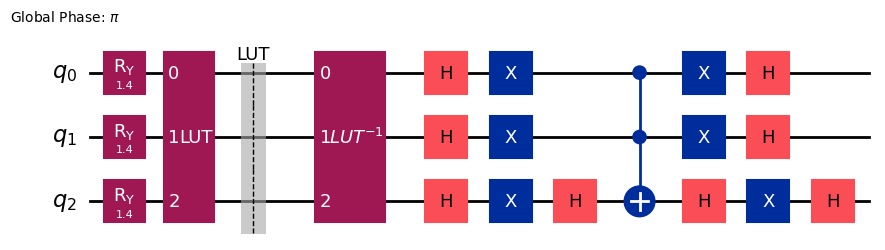
\includegraphics[scale=0.4]{improved_file_explorer.png}
	\captionof{figure}{Explorador de arquivos implementação}
	\label{fig:file-explorer}
\end{center}

Dessa forma, o arquivo procurado tem sua probabilidade maximizada pelo circuito, sendo apresentada a distribuição após $n$ medições.

\begin{center}
	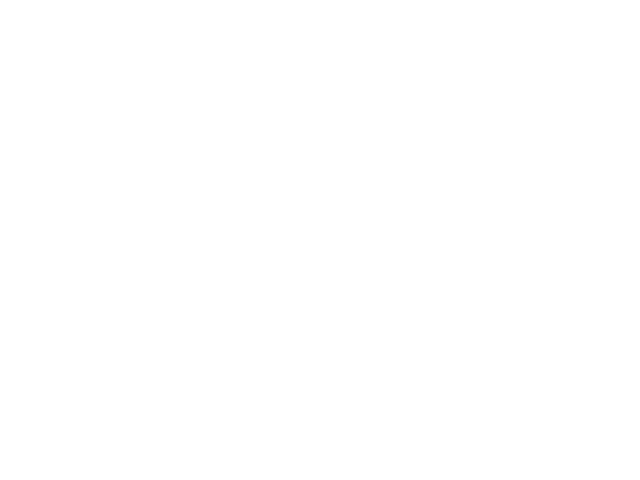
\includegraphics[scale=0.6]{AER-file-explorer-hist-new-grover-mapped-rotations.png}
	\captionof{figure}{Explorador de arquivos resultados - Qiskit AER ($shots=1000$)}
	\label{fig:file-explorer-hist}
\end{center}

\subsubsection{Resultados}

Para esse caso hipotético, certamente essa é um das melhores maneiras para fazer buscas dentre todos os arquivos armazenados.\\
Contudo, ao projetar esse modelo para um sistema clássico, tentando tomar proveito da computação quântica, essa não se mostra como a melhor opção. Isso acontece pois, guardar uma Look-Up-Table para os arquivos, e outra para cada ângulo de cada bit-string dentre as $2^{n}$ combinações, pode ser custoso e lento, além de requerer uma hash function com pouca probabilidade de colisão. Para diminuir esse overhead, poderia ser utilizado, simplesmente, o algoritmo de Grover sem maiores alterações, mas ainda assim seria necessário ter mapeado todos os arquivos em disco para a tabela. Assim, tomando como referência sistemas que utilizam o mapeamento de arquivos baseado em árvores ($O(log(n))$), esse método não apresenta ganho algum, além de possuir a probabilidade de não encontrar, ou retornar o arquivo errado.

\begin{center}
	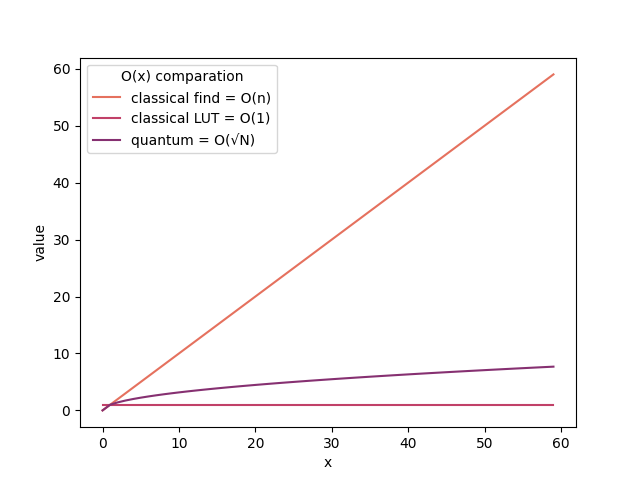
\includegraphics[scale=0.5]{algorithms-finding-comparation.png}
	\captionof{figure}{Comparação algoritmos usados na pesquisa}
	\label{fig:file-explorer-comparation-O}
\end{center}

Sendo assim, os algoritmos apresentados, são as melhores alternativas para serem utilizadas em um sistema que é, principalmente, quântico. Mas para casos de otimização clássica, deve ser utilizado apenas para complexidades $\ge O(n)$.


\subsection{Milhas para Quilômetros} \label{conversion}
O segundo problema testado, foi a conversão de milhas para quilômetros. Essa ideia se deu após a descoberta de um algoritmo capaz de calcular a sequência de Fibonacci usando circuitos quânticos, algoritmo essencial para esse projeto.

\subsubsection{Algoritmos usados}

\subsubsubsection{Algoritmo Quântico de Fibonacci}
A versão quântica usada para calcular Fibonacci foi apresentada em \cite{gilliam2020canonical} e  demonstra que, utilizando um circuito do qual coloca em superposição todas as bit-strings com $n$ qubits, e então realizando operações para remover valores que possuem $1$s consecutivos, é possível encontrar o valor $n$ na sequência.

\begin{center}
	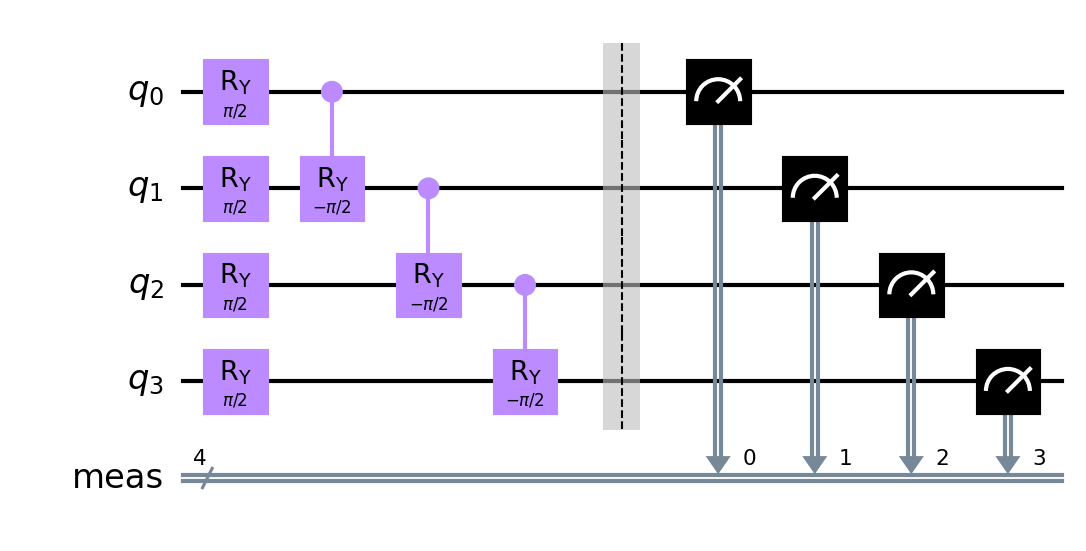
\includegraphics[scale=0.3]{fibonacci-circuit.png}
	\captionof{figure}{Exemplo Algoritmo Quântico de Fibonacci}
	\label{fig:fibonacci-circuit}
\end{center}

\begin{center}
	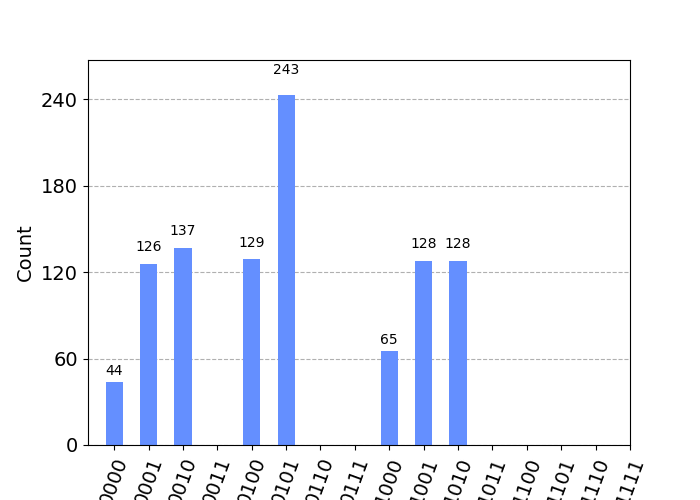
\includegraphics[scale=0.6]{fibonacci-4.png}
	\captionof{figure}{Resultado Fibonacci - F(4)}
	\label{fig:fibonacci-circuit-result}
\end{center}

Após executar o circuito, é necessário verificar a quantidade de bit-strings únicas que apareceram durante os experimentos. No exemplo em \ref{fig:fibonacci-circuit-result}, foram usados $4$ qubits para calcular $F(4)$. Assim, ao contar as bit-strings, temos $F(4) = 8$, retornando então o quarto valor da sequência (nesse caso, a sequência começa do valor $2$, seguindo dessa forma: $F(1)=2, F(2)=3, F(3)=5, F(4)=8, F(5)=13, F(6)=21, ...$). \\
Com isso, é possível usar esse circuito para computações de $F(n)$ utilizando $n$ qubits para encontrar o valor requisitado nessa mesma posição $n$.

\subsubsubsection{Aproximação de Milhas para Quilômetros usando Fibonacci}

Para aproximar o valor de milhas para quilômetros, podemos utilizar a sequência de Fibonacci com a seguinte relação: $F_{km} = F_{milhas}(n+1)$, sendo aqui $F$ a versão clássica de Fibonacci com $F(1) = 1$ e $F(2) = 2$. Dessa forma, se a posição $n$ é conhecida, valor aproximado em quilômetros será dado em $n+1$.


\begin{table}[!h]
	\begin{center}
		\begin{tabular}{ |c|c| } 
			\hline
			milhas & km \\
			\hline
			1 & 2 \\
			\hline
			2 & 3 \\
			\hline
			3 & 5 \\
			\hline
			5 & 8 \\
			\hline
		\end{tabular}
	\caption{valores aproximados de Milhas para Quilômetros}
	\end{center}
\end{table}

Valores não presentes na sequência, podem ser aproximados repartindo o valor em partes menores. Por exemplo, para transformar $10$ milhas em quilômetros, podemos fazer: $8 + 2 = 10miles \to F(5) + F(2) \to F(5+1) + F(2+1) =  13 + 3 = 16km$, aproximando então do valor mais preciso de $\approx 16.0934$


\subsubsection{Implementação do circuito}
Com essa formulação, o algoritmo final segue esse fluxo:

\begin{algorithm}[H]
	\begin{algorithmic}
		\State{partes = $quebraValor(valorDeEntrada)$}
		\For{parte in partes}
			\State{Aplique o Oracle $F(parte)$}
			\State{Faça as medições nos qubits}
			\State{Reset os qubits usados}
		\EndFor
		\State{verifique o resultado de cada bit-string}
		\State{Multiplique cada resultado com o valor $i$ correspondente}
			
	\end{algorithmic}
	\caption{Algoritmo quântico para a conversão}
	\label{alg:miles-to-km-quantum-algortihm}
\end{algorithm}


Nesse formato, é necessário pré-processamento utilizando um algoritmo clássico para dividir o número em partes menores. Este então, retorna tuplas mapeando a entrada para o valor $n_i$ e a quantidade de vezes que é necessário a sua aplicação $p$, $(n) \to ((n_1, p_1), (n_2, p_2), ...)$.\\
A partir disso, a parte quântica segue com a aplicação do algoritmo de Fibonacci em formato de Oracle no circuito para o valor $n_i$, em seguida as medições nos qubits usados pelo Oracle e por fim o reset deles, seguindo esse ciclo para cada valor $n$.\\
Após terminar, basta pegar os resultados, e, com um pouco de pós-processamento, agrupar as partes e multiplicar pelo seus valores $p$, retornando então o valor aproximado em quilômetros.

\begin{center}
	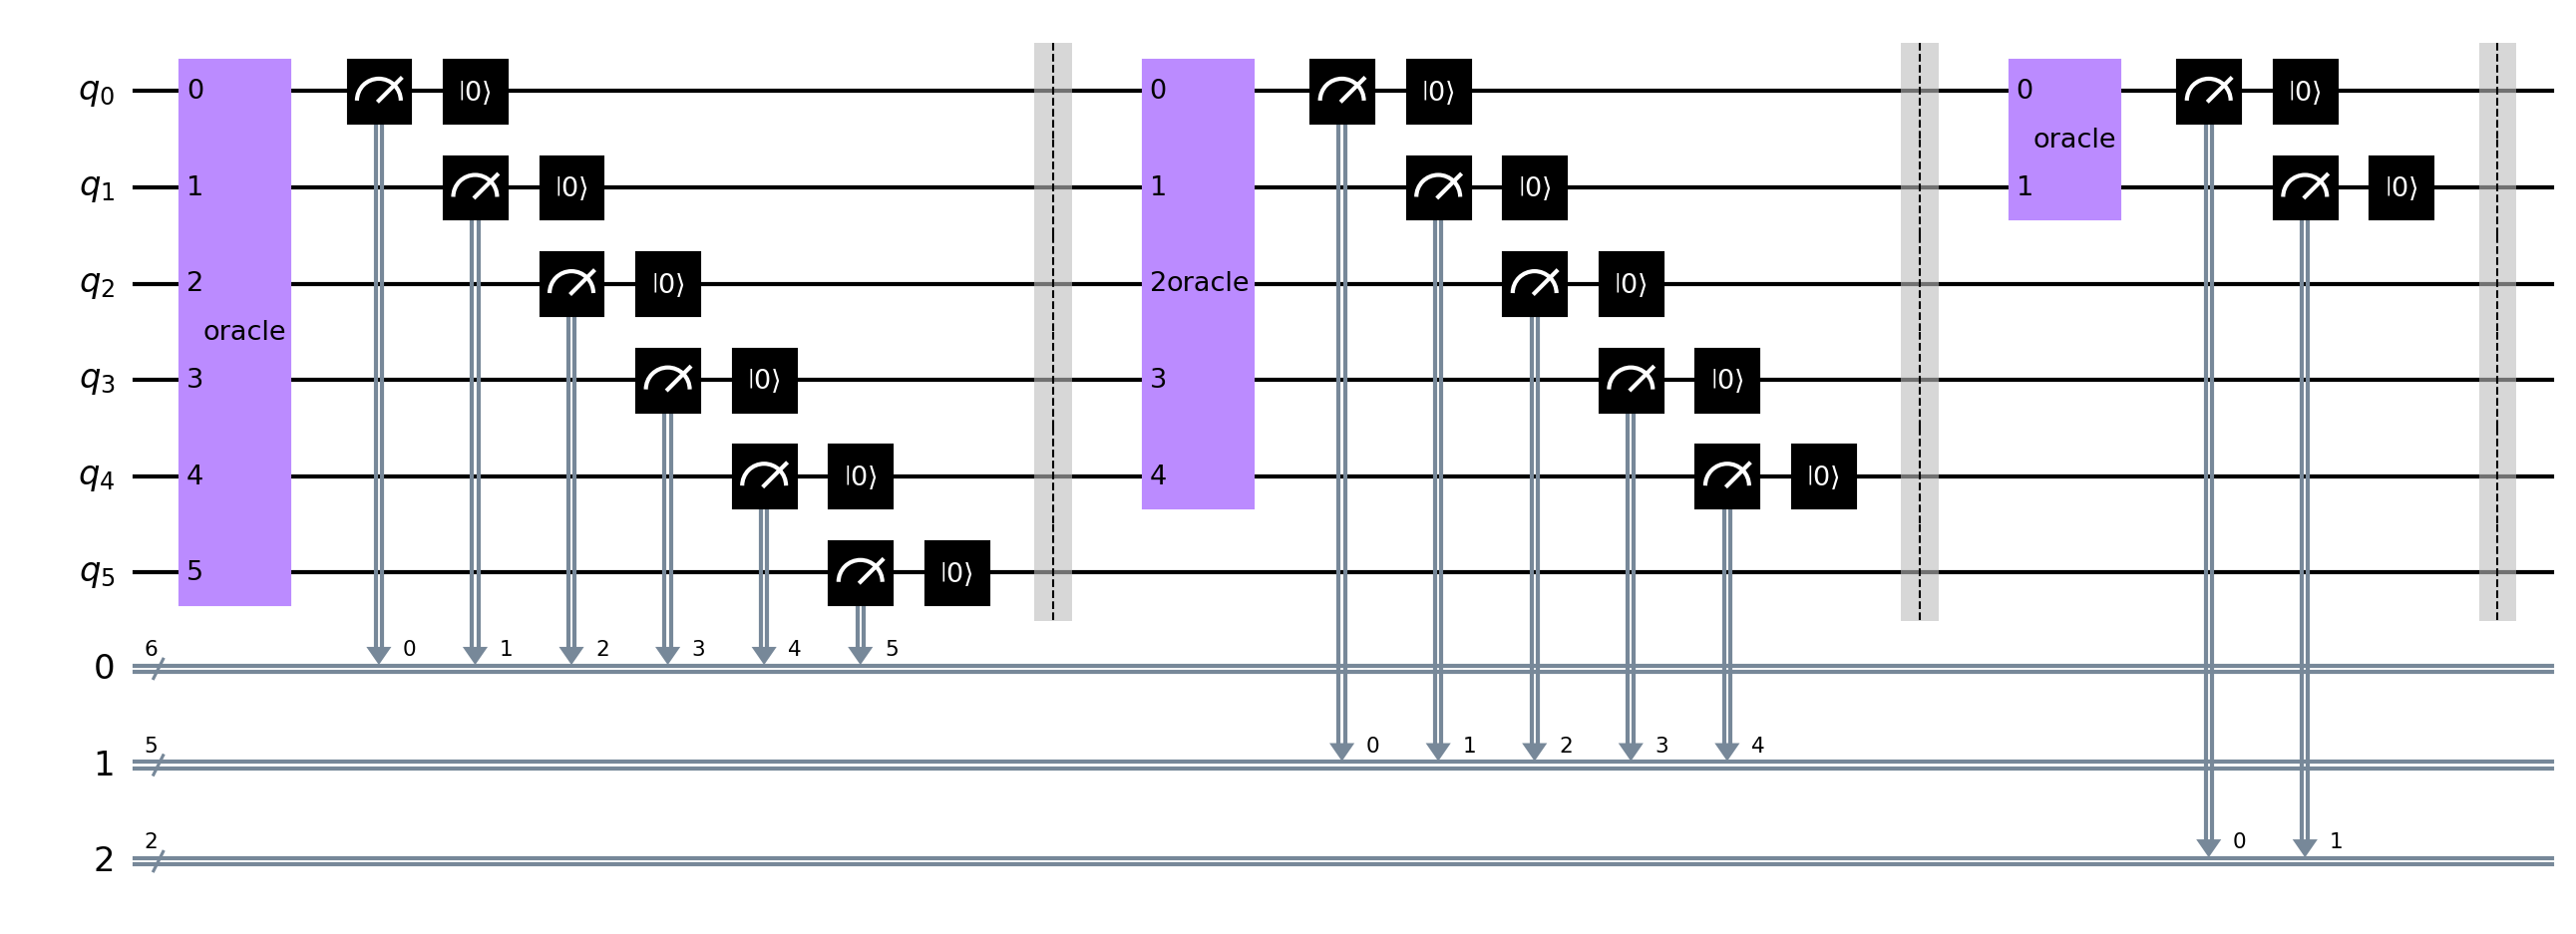
\includegraphics[scale=0.15]{number_breakdown_circuit.png}
	\captionof{figure}{Circuito de conversão}
	\label{fig:miles-km-circuit}
\end{center}

\subsubsection{Resultados}
Usando esse método, é possível alcançar os valores esperados. Contudo existem alguns pontos que tornam esse método inviável:

\begin{enumerate}

\item{\textbf{Quantidade necessária de medições e tempo de execução}}\\
Para cada medição do circuito, é necessária uma quantidade alta de \emph{shots} (valores entre $5000$ e $10000$ foram testados localmente usando o Qiskit AER e, para os testes no hardware da IBM, foram usados apenas $1000$ por questões de extrema demora e erros durante os experimentos) para alcançar melhores resultados, aumentando também o tempo necessário para finalizar a execução.

\begin{center}
	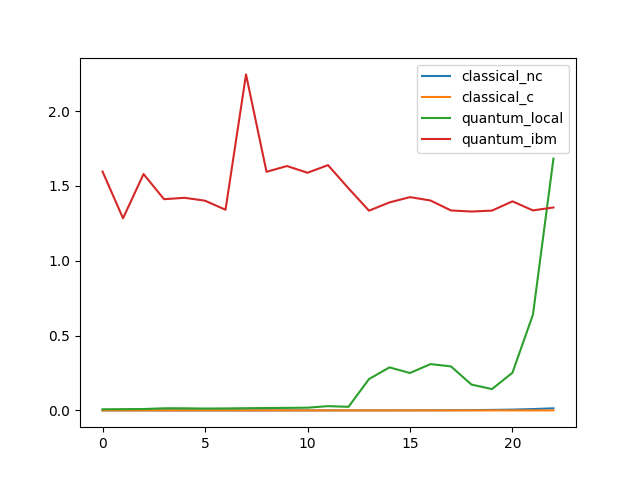
\includegraphics[scale=0.6]{comparison_miles_to_km.png}
	\captionof{figure}{Comparação tempos de execução}
	\label{fig:comparasion-miles-km-time}
\end{center}

Como mostrado em \ref{fig:comparasion-miles-km-time}, o tempo das versões clássicas, com e sem memoization, possuem tempos praticamente constantes em relação as versões quânticas.


\item{\textbf{Erros}}\\
Como a maioria dos algoritmos Quânticos da era NISQ(noisy intermediate-scale quantum), os erros também estão presentes, e por serem utilizados inúmeros gates multi-qubits, esses erros podem ainda se intensificar de acordo com hardware usado.

\item{\textbf{Imprecisão}}\\
\begin{center}
	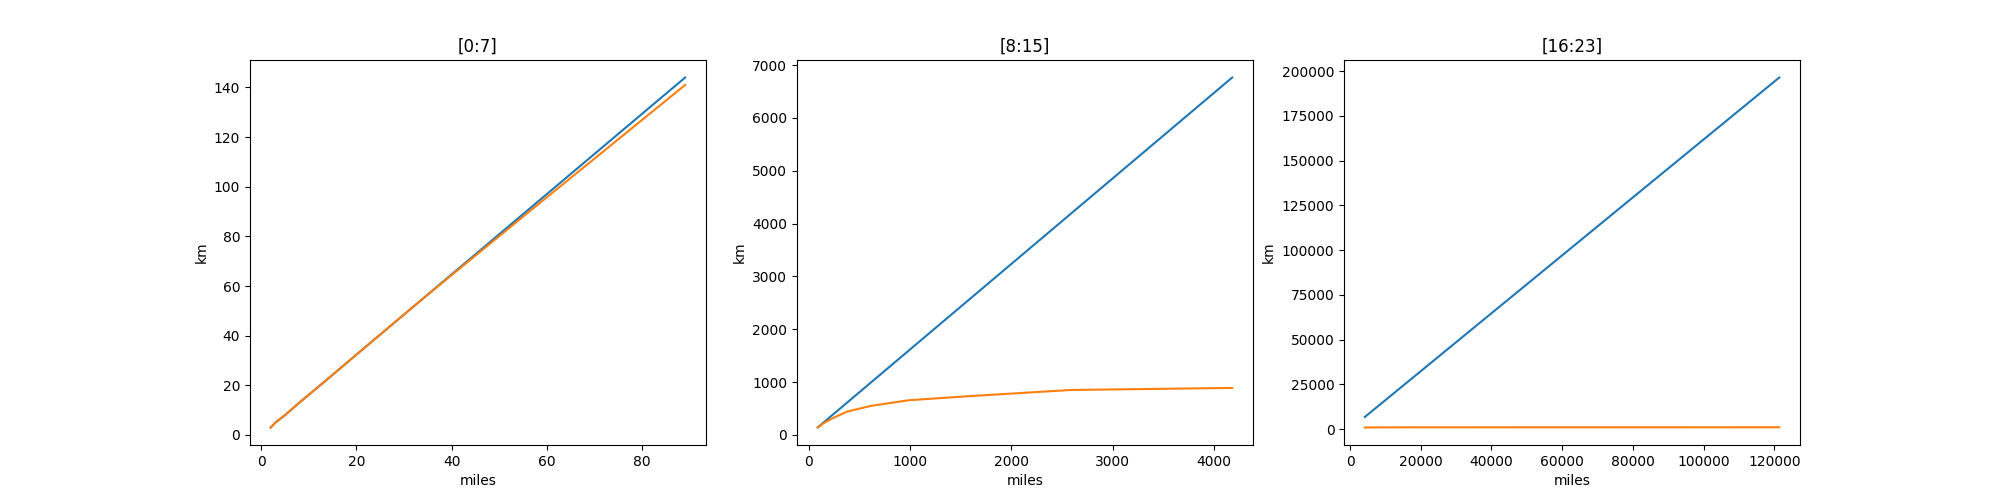
\includegraphics[scale=0.4]{miles_to_km_defiance.png}
	\captionof{figure}{Comparação resultados versão clássica e quântica}
	\label{fig:values-miles-km-quantum}
\end{center}

Como mostrado em \ref{fig:values-miles-km-quantum}, valores pequenos possuem uma boa precisão com os números esperados, mas a partir de certo ponto, eles começam a se distanciar e perdem totalmente a precisão.

\item{\textbf{Necessidade de intervenção clássica}}\\
Por requisitar pré e pós processamento clássico e apenas uma pequena parcela ser de fato processamento quântico, a necessidade de utilizar esse algoritmo se reduz a zero. 

\end{enumerate}

Sendo assim, esse algoritmo não consegue se sair bem como a versão clássica, além de ser mais custoso na maioria dos casos. Para evoluir essa implementação, será necessário remodelá-lo para um versão com pouca, ou nenhuma, computação clássica, priorizando a maneira como dados podem ser encodados e transformados no circuito.

\subsection{Torres de Hanoi} \label{hanoi}
Para a criação das torres de Hanoi, foi pensado em uma maneira de encodar a posição dos discos na torre utilizando seus valores binários e o Phase Oracle como meio de armazenamento.

\subsubsection{Implementação}
Para esse projeto, são necessários $(\floor{\log_2{x}} + 1) * 3$ qubits, sendo $x$ o número de discos. Estes seguem a ordem $\ket{t_{n-1} t_{n-2} ... t_0}\ket{a_{n-1} a_{n-2} ... a_0}\ket{s_{n-1} s_{n-2} ... s_0}$, sendo $s$,$a$,$t$ a primeira, segunda e última torre respectivamente, e $n = {{n \space qubits} \over 3}$.\\
Com essa configuração, os números de $1$ à $x$ são codificados em seu formato binário nos qubits $s$, utilizando a fase global $\pi$. Em seguida, são realizadas operações de $swap$ bit-a-bit para mover os valores dos $n$ qubits menos significativos para os $n$ mais significativos.\\
Para realizar essas operações, é necessário pré-calcular, classicamente, a sequência de movimentos usados  \cite{ldiaandr_2021_tower} \cite{diptokarmakar47_2019_how} \cite{a2020_towers}  \cite{geeksforgeeks_2014_program}. Dessa forma, essa versão quântica age como um jogador com uma lista de passos a serem seguidos, executando-os um-a-um.

\begin{center}
	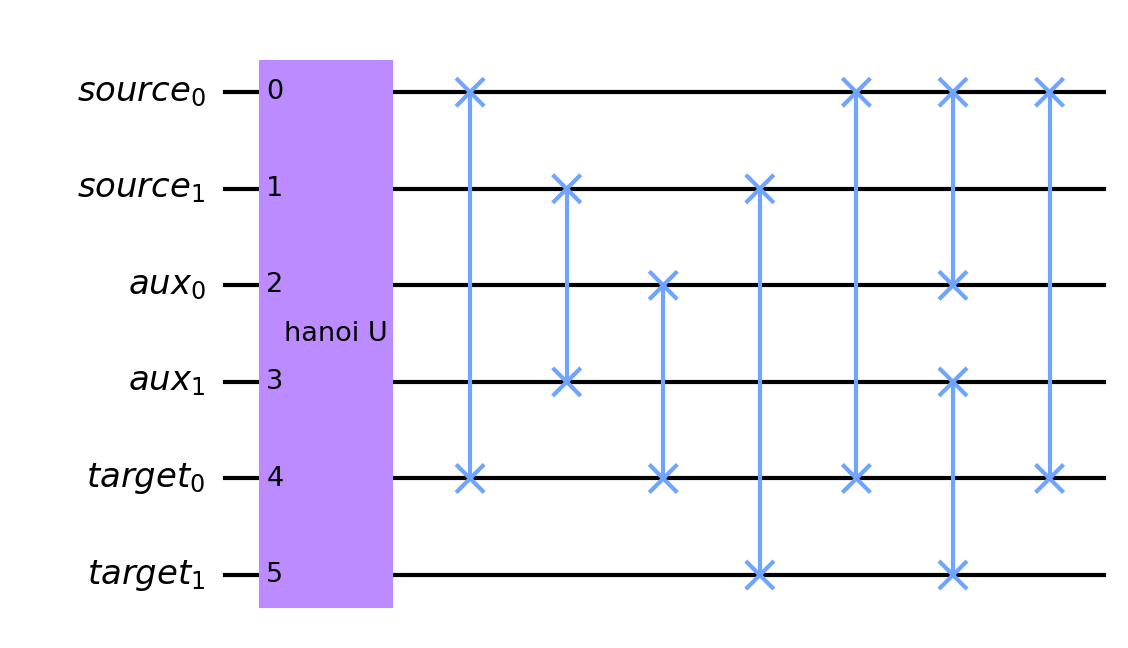
\includegraphics[scale=0.3]{hanoi_3_discs.png}
	\captionof{figure}{Torre de Hanoi com 3 discos}
	\label{fig:hanoi}
\end{center}

Nesse circuito, pode-se utilizar algoritmos adicionar, como o algoritmo de Grover, para verificar o resultado, ou executar outras operações nos valores.

\begin{center}
	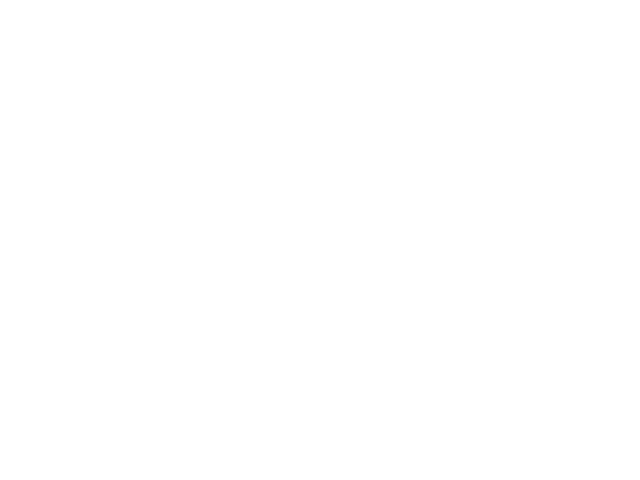
\includegraphics[scale=0.5]{result_hanoi_3_discs.png}
	\captionof{figure}{Resultado usando Grover - Torre de Hanoi com 3 discos}
	\label{fig:hanoi-result}
\end{center}

Em \ref{fig:hanoi-result}, os $3$ maiores resultados obtidos são as bit-strings com $01$, $10$ e $11$ nos bits mais significativos. Sendo assim, o resultado esperado para uma torre com 3 discos, foi atingido.

\subsubsection{Resultados}
Nessa versão, é seguida a mesma sequência do algoritmo clássico, necessitando, inclusive, de pré-processamento para conseguir a sequência de ações.\\
Em uma versão clássica, o movimento de retirar um disco de uma torre e move-lo para a próxima requer também esse pré-processamento, podendo ser realizado um-a-um ou tudo de uma vez antes da partida. Dessa forma, a versão clássica e quântica se igualam, não tendo ganhos ou perdas expressivas.

\subsection{Buckshot Roulette} \label{buckshot}
\emph{Buckshot Roulette} é um jogo de computador feito pelo desenvolvedor \href{https://mikeklubnika.itch.io/}{Mike Klubnika}, tomando como base a premissa de reinventar a infame roleta russa. No jogo, você é desafiado por um demônio (dealer), e caso você ganhe, uma recompensa lhe será dado, caso contrário o jogo reinicia e você pode tentar novamente.\\
Nesse projeto, foi tomado como objetivo analisar a primeira rodado do jogo e tentar encontrar a melhor estratégia para maximizar os ganhos do jogador. O motivo da escolha da primeira rodada se dá pela sua simplicidade, sendo direto ao ponto, sem power-ups ou fatores que dificultariam as simulações, mas, ainda assim, mantendo a essência do jogo.

\subsubsection{Dinâmica}
Na rodada, são colocadas $2$ balas falsas e $1$ bala verdadeira na arma, sendo o player o primeiro a jogar. Ambos os jogadores podem escolher entre atirar em si mesmo, ou em seu oponente. Assim, a próxima ação é estritamente depende das probabilidades de ser uma bala real ou falsa. A partir dai, a dinâmica funciona da seguinte forma: 

\begin{algorithm}[H]
	\begin{algorithmic}
		\If{jogador escolhe atirar no dealer}
			\If{bala for real}
				\State{Jogador ganha a rodada}
			\Else
				\State{Dealer joga a próxima}
			\EndIf
		\Else
			\If{bala for real}
				\State{Jogador perde}
			\Else
				\State{Player joga a próxima}
			\EndIf
		\EndIf

	\end{algorithmic}
	\caption{Possíveis jogadas}
	\label{alg:buckshot-roulette}
\end{algorithm}

Essa dinâmica se repete a cada jogada, sendo válida tanto para o dealer, como para o player.


\subsubsection{Versão clássica}
Para entender melhor a dinâmica, é possível representar cada ação e suas consequências em formato de árvore. Dessa forma, cada jogada leva a partida para mais próximo do fim.


\begin{center}
	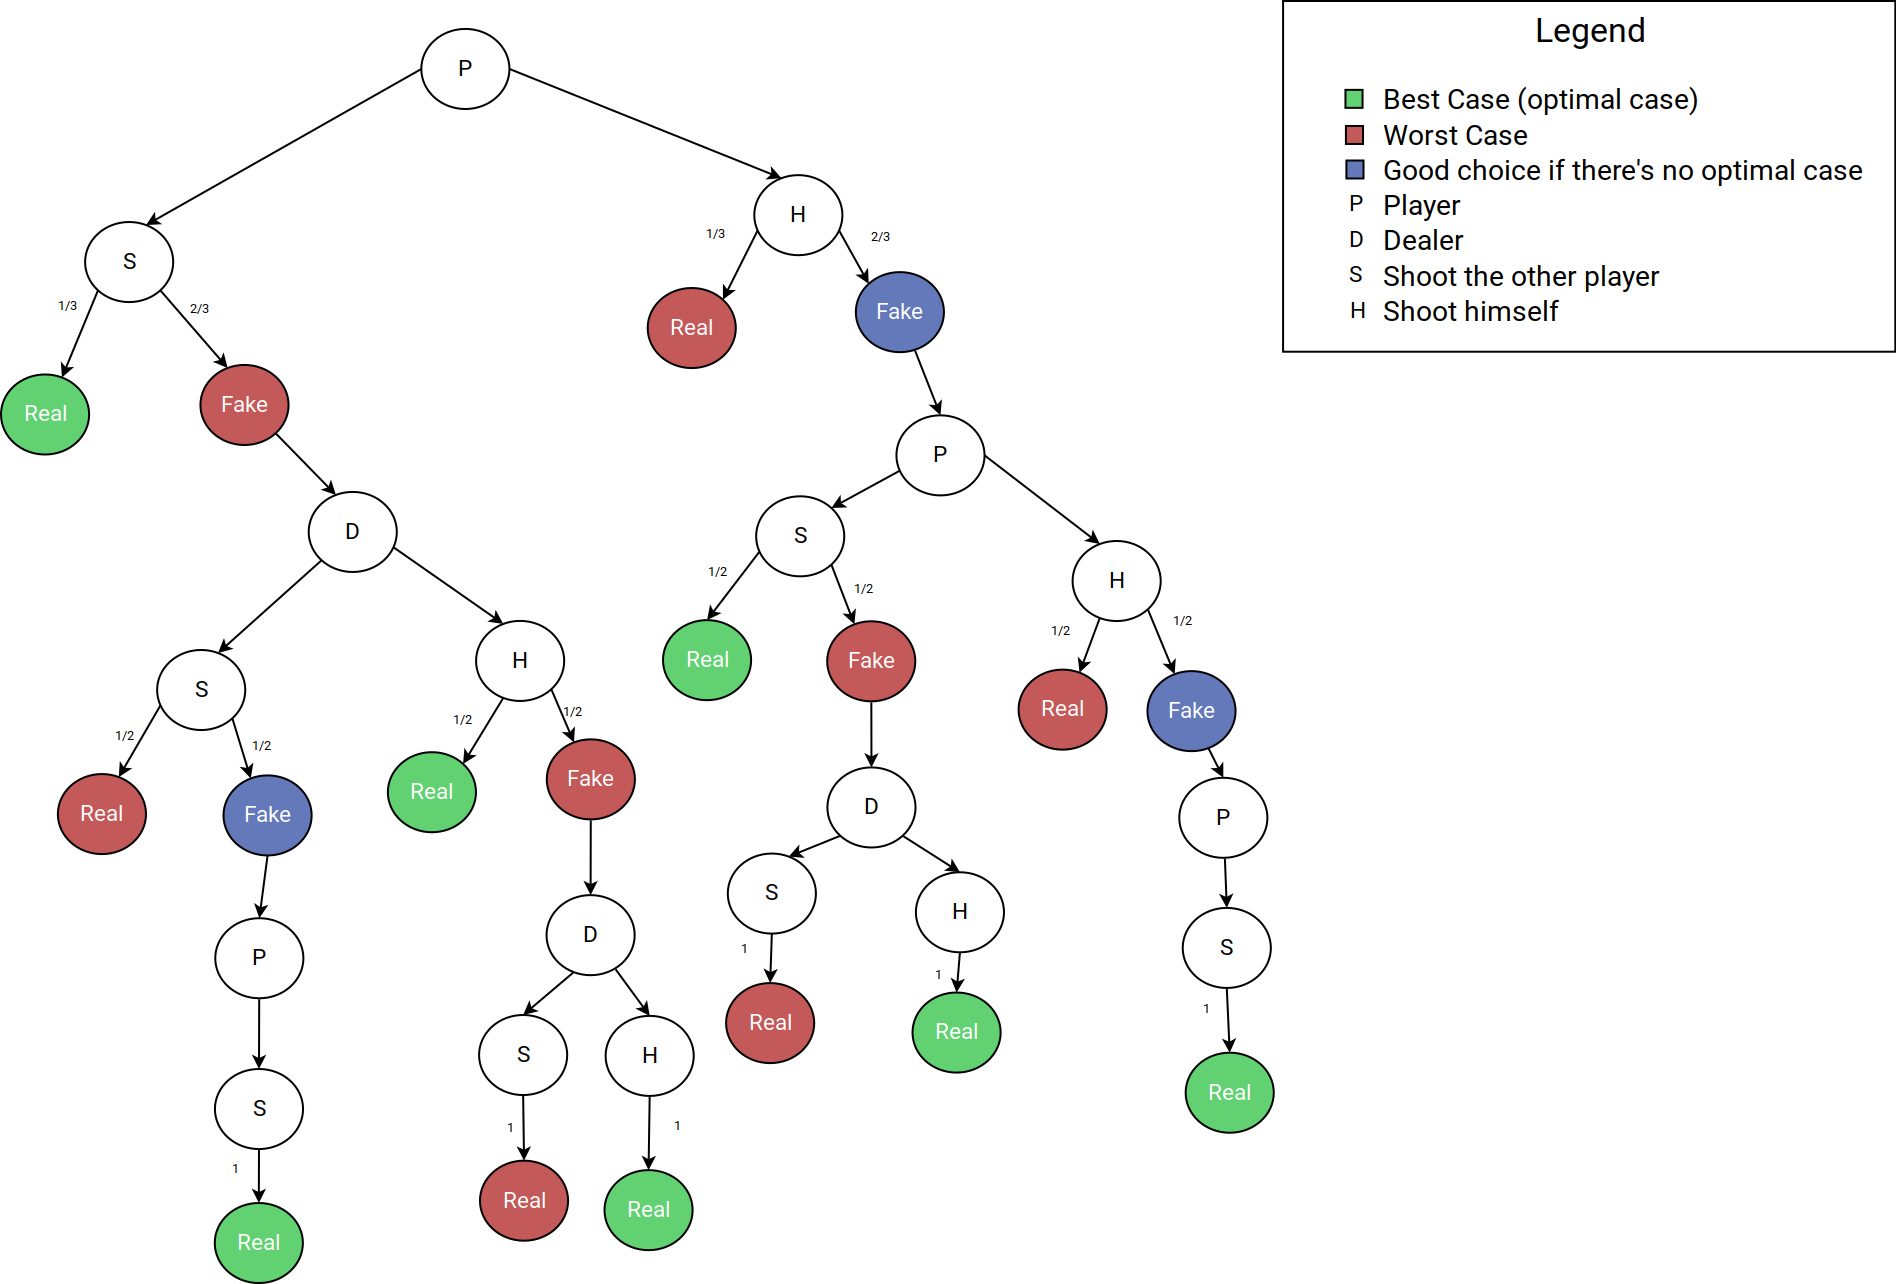
\includegraphics[scale=0.2]{buckshot-roulette-diagram.png}
	\captionof{figure}{Buckshot Roulette diagrama de árvore}
	\label{fig:classical-model-bckr}
\end{center}

Nessa estrutura, é previsto que o jogador seja um agente racional, e o dealer uma máquina com ações aleatórias. Assim, o jogador sempre visa o seu próprio benefício, enquanto o dealer age pela sorte.Tal comportamento pode ser visto nas folhas da árvore do qual, sempre que o player é o próximo jogador, sua ação é apenas atirar no adversário, enquanto o dealer ainda possui a possibilidade de entregar o jogo atirando em si próprio, mesmo havendo apenas uma bala na arma e, pela lógica do jogo, ser uma bala verdadeira.\\
Seguindo essa estrutura, podemos simular os possíveis caminhos e verificar a melhor estratégia.

\begin{center}
	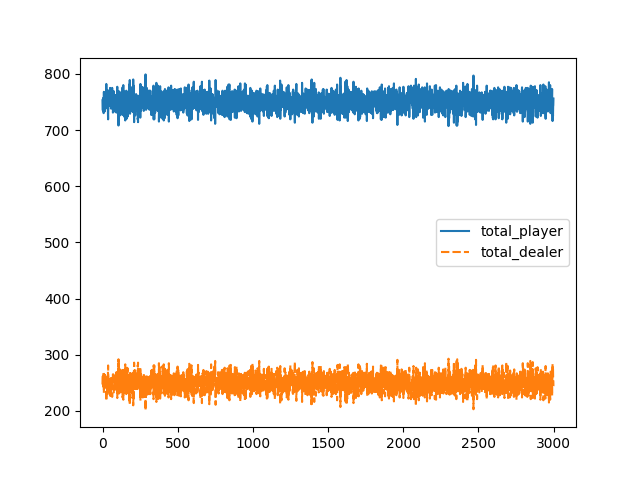
\includegraphics[scale=0.6]{optimal_player_strategy.png}
	\captionof{figure}{Buckshot Roulette clássico - melhor estratégia}
	\label{fig:classical-model-bckr-optimal-strategy}
\end{center}

Após testar os caminhos possíveis, o melhor resultado obtido foi esse apresentado acima em \ref{fig:classical-model-bckr-optimal-strategy}. Com um pouco de investigação, foi possível entender que essa estratégia se baseia no jogador começar atirando no dealer. Isso acontece, pois, ao seguir tal caminho, ele tem uma chance a menos de perder a rodada ao atirar em si mesmo logo no começo da partida.

\begin{table}[!h]
	\begin{center}
		\begin{tabular}{ |c|c|c|c| } 
			\hline
			rodada & ação & resultado da ação & resultado da partida \\
			\hline
			1 & player atira no dealer  & real & player ganha\\
			\hline
			1 & player atira no dealer  & fake & -\\
			\hline
			2 & dealer atira no player  & real & dealer ganha\\
			\hline
			2 & dealer atira no player  & fake & -\\
			\hline
			2 & dealer atira nele mesmo  & real & player ganha\\
			\hline
			2 & dealer atira nele mesmo  & fake & -\\
			\hline
			3 & player atira no dealer  & real & player ganha\\
			\hline
			3 & dealer atira no player & real & dealer ganha\\
			\hline
			3 & dealer atira nele mesmo  & real & player ganha\\
			\hline
		\end{tabular}
		\caption{melhor estratégia - possíveis resultados}
	\end{center}
\end{table}

\subsubsection{Versão quântica}
Para a versão quântica, um circuito foi modelado imitando o funcionamento do game. Nesse algoritmo, um Oracle foi usado para cada jogador, implementando internamente sua estratégia.

\begin{center}
	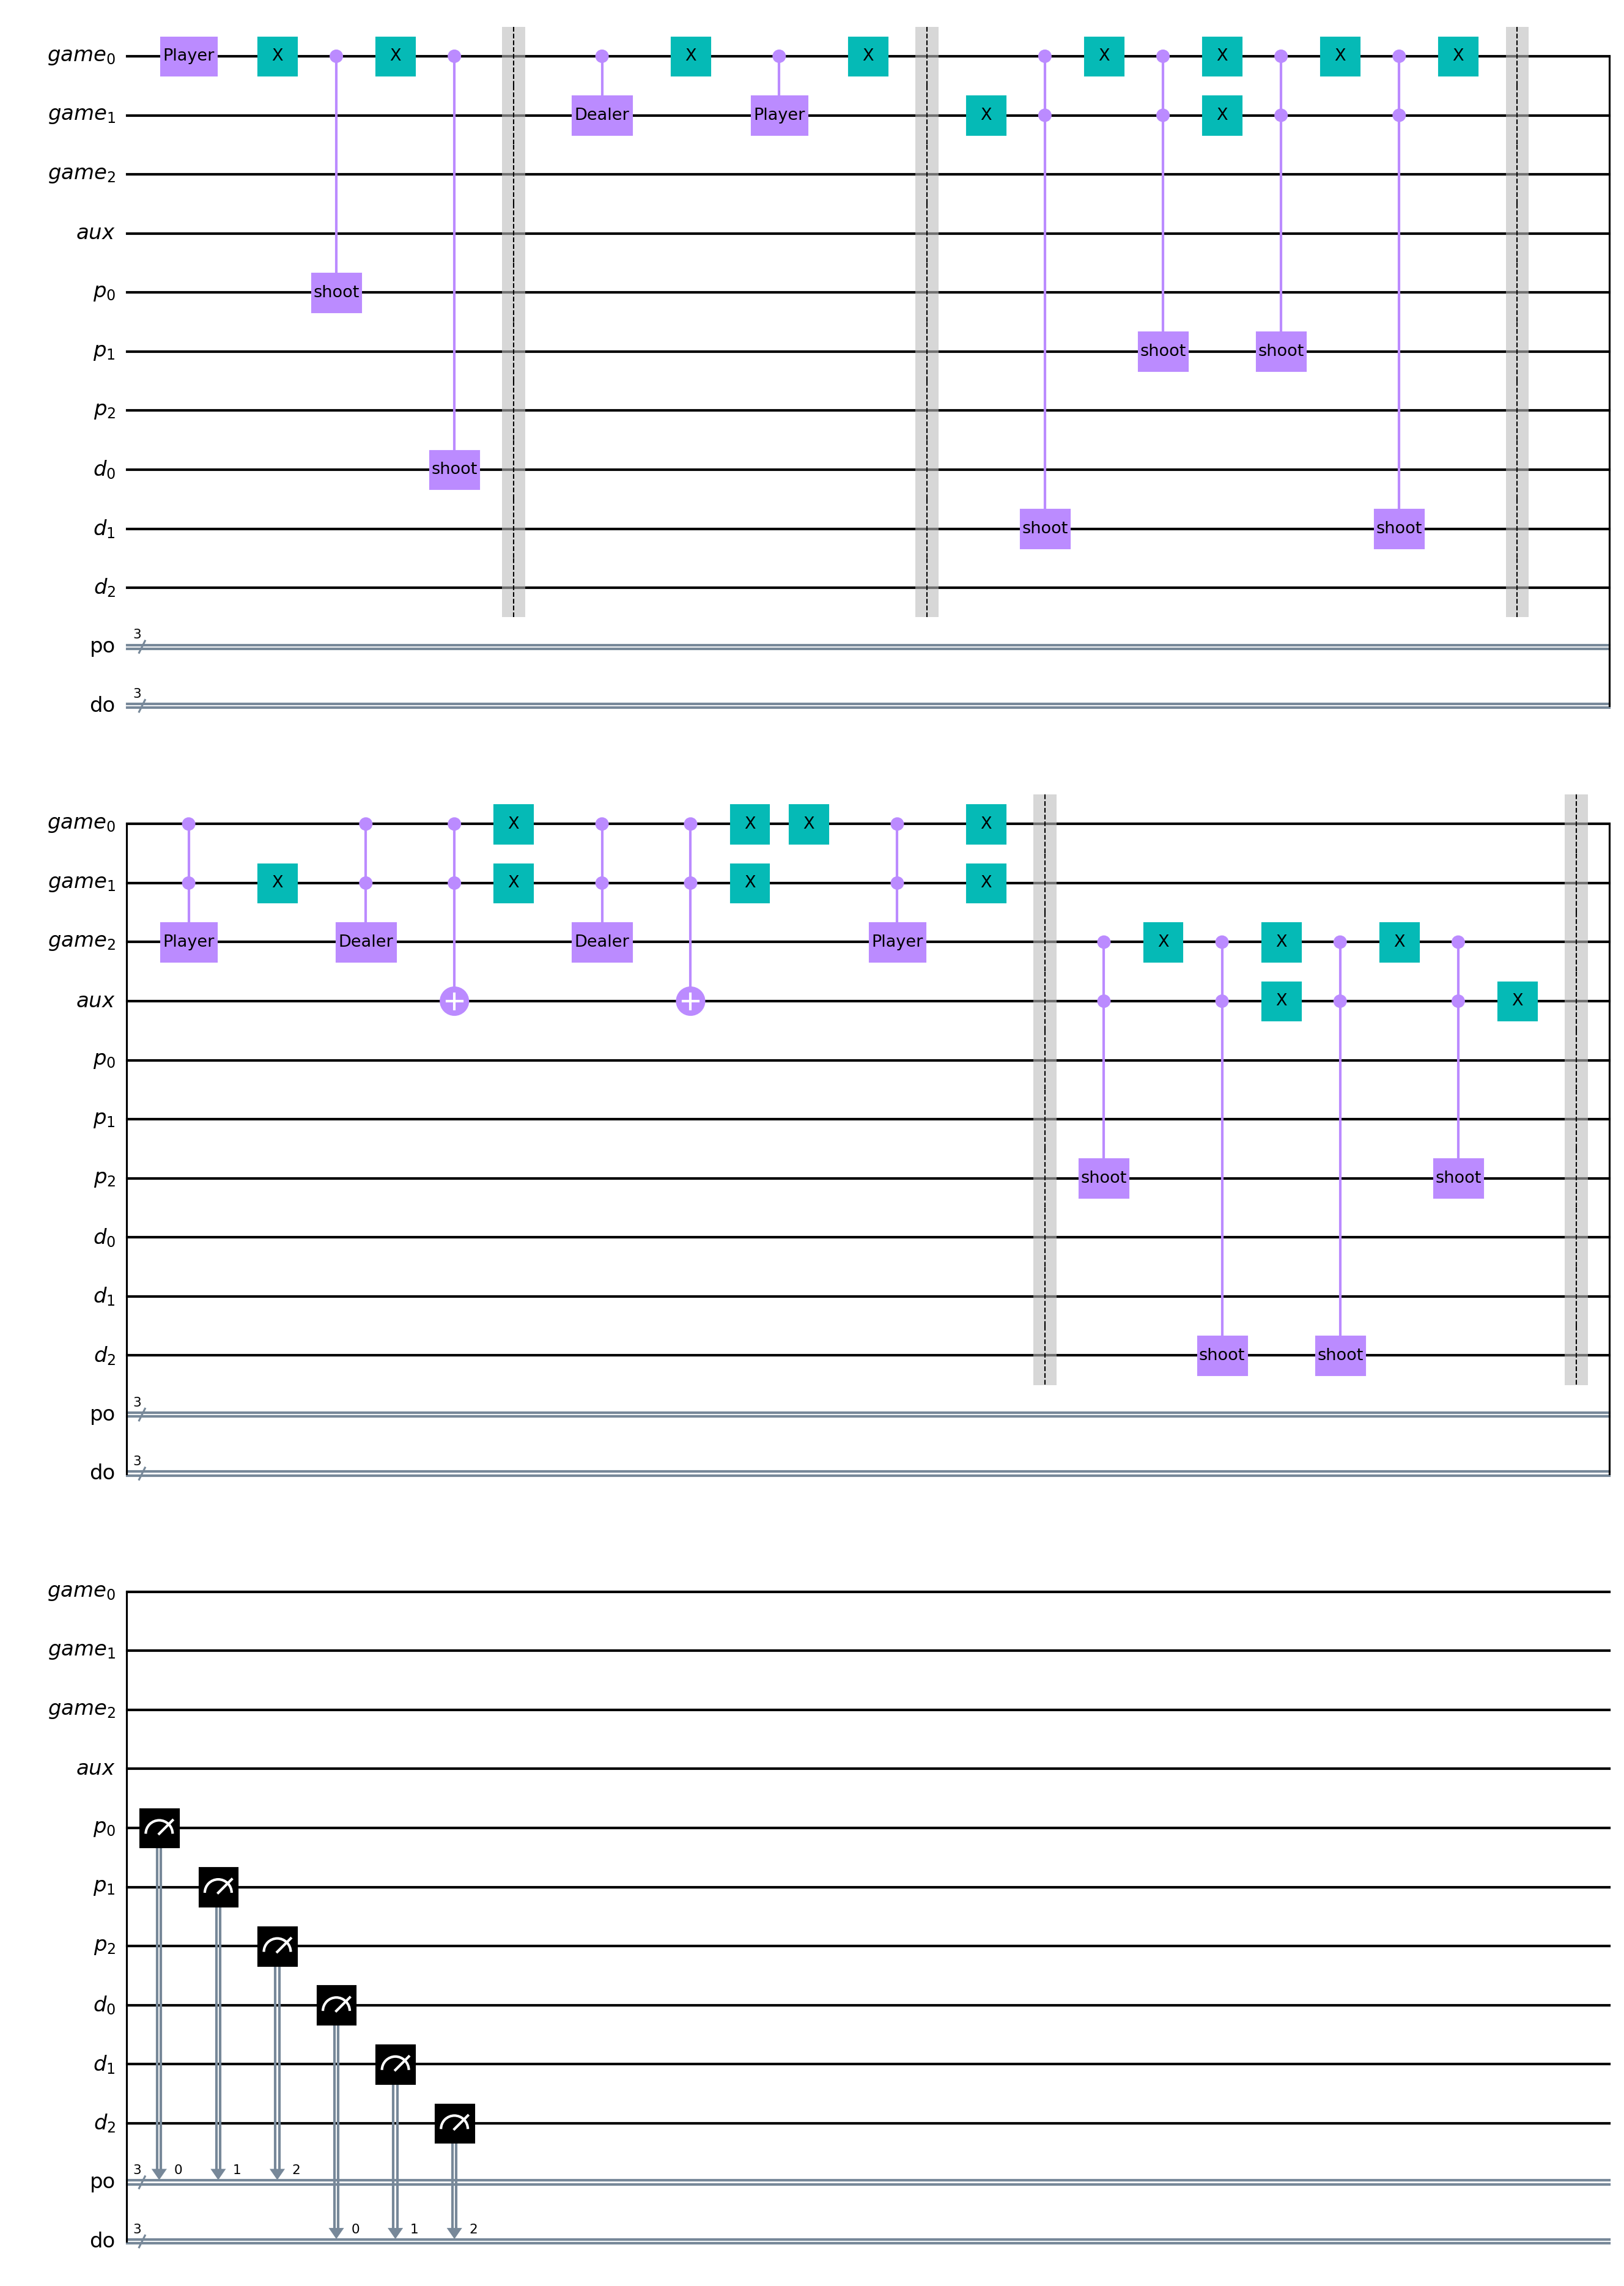
\includegraphics[scale=0.3]{quantum_buckshot_roulette.png}
	\captionof{figure}{Circuito para o Buckshot Roulette}
	\label{fig:bckr-circuit}
\end{center}

Além disso, para encontrar a estratégia, foram inseridos dois parâmetros dentro do Oracle do player, sendo possível configurar qualquer valor $\theta$ e $\phi$ para modificar a rotação na Bloch Sphere.\\
Após verificar os possíveis valores, a rotação que entregou o melhor resultado foi $\theta\approx 3.0853981633974477, \phi\approx3.7853981633974474$ radianos. Usando essa estratégia, os resultados foram semelhantes a versão clássica.

\begin{center}
	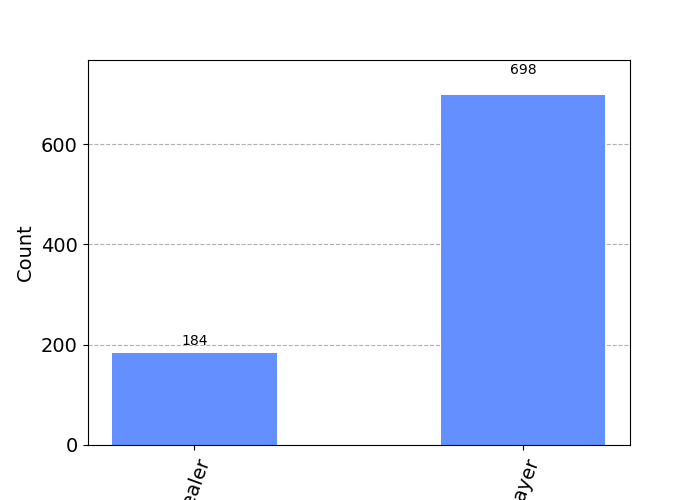
\includegraphics[scale=0.6]{final_buckshot_roulette_quantum_optimal_strategy.png}
	\captionof{figure}{Resultado Buckshot Roulette quântico - Qiskit AER}
	\label{fig:bckr-circuit-result}
\end{center}

Observando a Bloch Sphere do estado gerado por essa rotação, é possível ver também que a estratégia se aproxima da versão clássica, com o player preferindo atirar no dealer a maior parte do tempo (o valor $1$ representa atirar no outro jogador e $0$ em si mesmo).

\begin{center}
	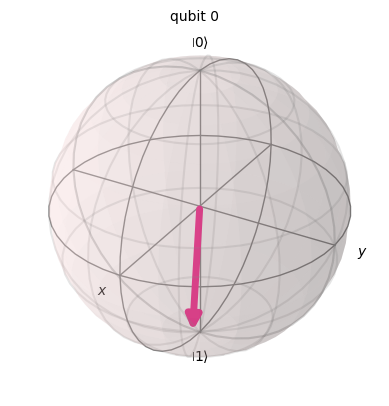
\includegraphics[scale=0.6]{player_optimal_strategy_bloch.png}
	\captionof{figure}{Melhor estratégia Buckshot Roulette quântico - Bloch Sphere}
	\label{fig:bckr-bloch-sphere-best-strategy}
\end{center}

Como uma última nota sobre o circuito, no exemplo \ref{fig:bckr-circuit-result}, o total de partidas ganhas por cada jogador não chega ao total jogado (nesse caso $1000$ partidas foram simuladas). Isso acontece devido ao design do circuito, o qual não é possível verificar a jogada do player anterior, acarretando na continuação do jogo mesmo que um dos players já tenha perdido, o que cria a necessidade do uso de pós processamento para limpar os resultados inválidos.

\subsubsection{Conclusões}
Para esse problema, não há uma competição certa entre as duas versões, já que uma é diretamente inspirada na outra. Contudo, a versão quântica possui ainda a possibilidade de explorar mais valores do que a versão clássica, deixando o player mais aberto a escolha de novas estratégias, o que pode ser visto como um ponto a favor da versão quântica.\\
Em suma, ambos as simulações atingiram o mesmo resultado e foi demonstrado que é possível usar o quantum Oracle como uma representação de um player dentro do circuito.

\subsection{QRAM} \label{qram}
Por fim, o último projeto realizado foi o de uma \emph{QRAM} utilizando os Oracles. Nessa versão, foi testado a criação de \emph{QROMs} (com dados estáticos dentro), e uma possível maneira de utilizar uma QRAM hábil para escrita.\\
Neste projeto, foi tido como objetivo o armazenamento de estados quânticos (superposições), e não apenas de bit-strings clássicas. Isso pois, para garantir a real eficiência da computação quântica, a superposição é indispensável, e seu armazenamento pode ser um ponto chave para algoritmos melhores.

\subsubsection{QROM}
Para a QROM, são utilizados $n$ qubits para o barramento de endereços e $m$ qubits para a o barramento de dados, sem a necessidade desses valores estarem correlacionados, podendo assim ser utilizado, por exemplo, $n=3; m=10$. Nessa estrutura, podemos mapear diversas superposições diferentes e aplicá-las quando certo endereço for chamado. Sendo assim, o algoritmo armazena os valores a partir da configuração de gates controlados interiores ao Oracle, criando uma superposição apenas quando certo valor de entrada é inserido, seguindo o formato: ${\ket{0}^{\otimes m}} {\ket{a_{n-1} a_{n-2} ... a_0}}$.

\begin{center}
	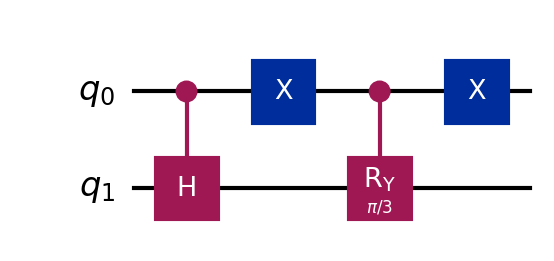
\includegraphics[scale=0.5]{qrom_1.png}
	\captionof{figure}{Exemplo circuito - QROM}
	\label{fig:qrom}
\end{center}


Em \ref{fig:qrom}, $q_{0}$ age como o barramento de endereços, enquanto $q_{1}$ como o barramento de dados. Aqui configuramos para mapear o endereço $0 \to RY({\pi\over{3}})$ e $1 \to H$. Sendo assim, para $n$ qubits no barramento de endereços é possível mapear para $2^{n}$ estados, e com os $m$ qubits é possível criar estados mais complexos aumentando sua quantidade e utilizando outros gates acionados para um mesmo endereço. \\
A partir da abstração desse circuito para um Oracle,é possível utilizar a QROM em um circuito maior, chamando-o novamente sempre que for necessário um certo estado. Além disso, no formato de Oracle, há a possibilidade de colocar os endereços em superposição e ter uma mistura de estados na saída.

\begin{center}
	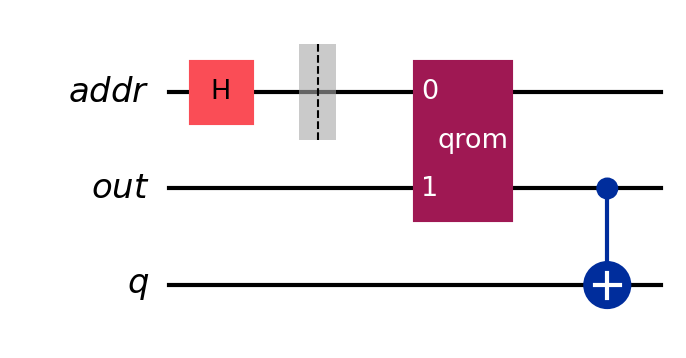
\includegraphics[scale=0.5]{qrom_1_usage.png}
	\captionof{figure}{Exemplo circuito usando a QROM com endereços em superposição}
	\label{fig:qrom-usage}
\end{center}

Nesse exemplo \ref{fig:qrom-usage}, os endereços são colocados em superposição no qubit \emph{addr} e assim os estados em internos do Oracle são colocados em uma sobreposição de $50-50$ no qubit \emph{out}. Com isso, pode-se aproveitar do resultado de \emph{out} em outros qubits, como nesse caso o qubit \emph{q}.\\
Contudo, devido ao no-cloning-theorem, não é possível copiar esse estado para outro qubit alvo. Sendo assim, não é possível ter dois qubits com o mesmo estado a partir daquele armazenado, podemos apenas pegar o resultado de uma superposição e utilizar o valor binário como trigger para outra operação.\\
Uma opção para solucionar isso, é utilizar o teleporte quântico, destruindo assim o estado interno do Oracle e movendo-o para outro qubit desejado.

\subsubsection{QRAM}
Para criar uma QRAM com a possibilidade de escrita, o teleporte quântico, já citado anteriormente, é um caminho para isso. Com ele, podemos ter $n$ qubits, sendo cada qubit um endereço único, e utilizar do teleporte para mover um estado que estava no circuito, para o domínio da QRAM.

 \begin{center}
 	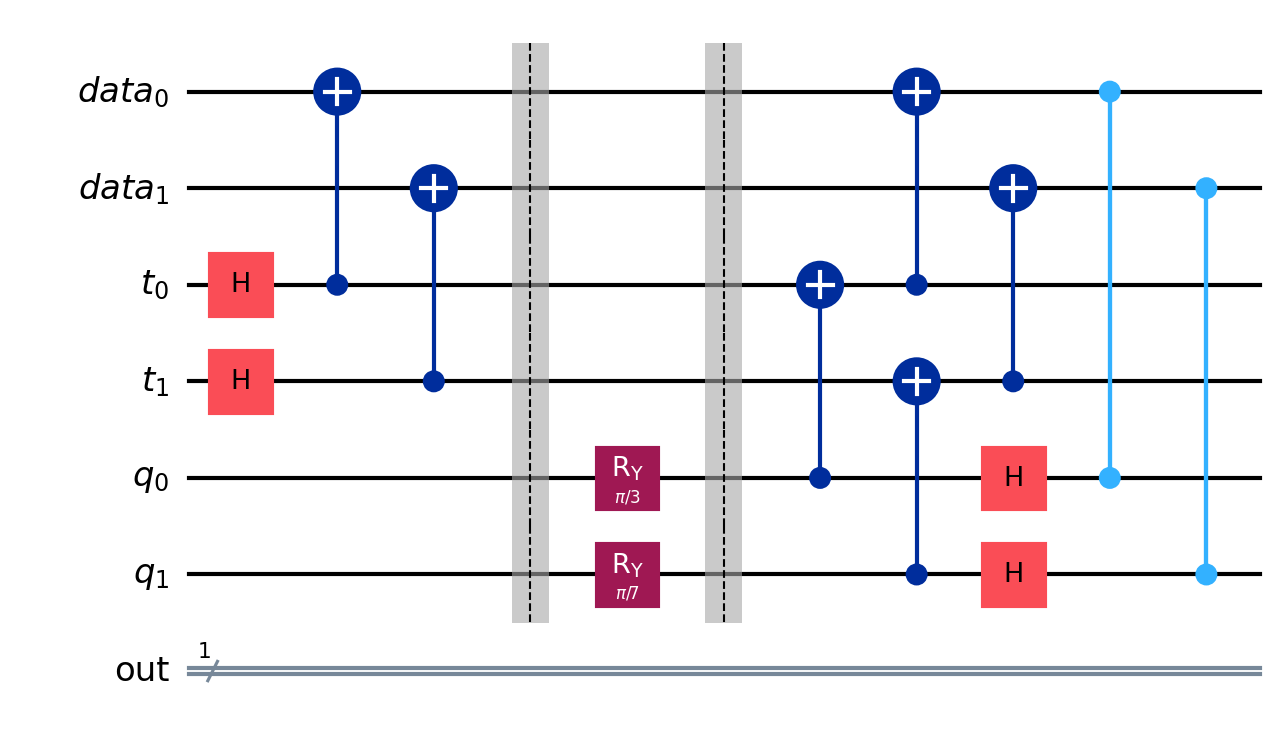
\includegraphics[scale=0.4]{qram.png}
 	\captionof{figure}{Exemplo circuito - QRAM}
 	\label{fig:qram}
 \end{center}

Aqui, os $n$ qubits agem tanto como endereços quanto dados (qubits \emph{data}). Além disso, são necessários mais $n$ qubits para o teleporte (qubits \emph{t}).\\
Com isso, é possível ver que o circuito cresce de forma linear a medida que mais endereços são requisitados, sendo assim $O(2*n)$ em relação à quantidade de qubits total.\\
Na configuração acima \ref{fig:qram}, é possível sobre-escrever valores, assim como interferir com outras superposições apenas teleportando novos valores para o qubit $i$. Dessa forma, podemos criar uma memória menor e, conforme necessário, remover e adicionar outros valores.

\subsubsection{Conclusões}
Com esse projeto, e com a literatura usada \cite{jaques2023qram}\cite{Giovannetti_2008}, é possível entender que criar versões quânticas de memória é uma tarefa desafiadora, e ainda não é possível tomar proveito de todo o seu potencial usando as superposições e estados de outras bases a não ser a base computacional $({0,1})$. Fatores como, complexidade de mapear dados, complexidade de utilizar a memória (já que é necessário reaplica-lá toda vez que for requisitado seu uso), no-cloning-theorem, decorrência, etc. Influenciam diretamente na possibilidade de sua criação.Mesmo sendo possível implementar pequenos circuitos que agem como memória, como os mostrados aqui, ainda não é usual e muito menos universal para qualquer tipo de máquina quântica.\\
Além disso, por esses fatores, a QRAM, pode dificultar a execução de múltiplas tarefas, uma vez que o valor presente nela não pode ser copiado, e ao move-lo para outro qubit, o valor anterior da QRAM é completamente destruído.\\
Como mostrado na literatura, para resolver esses problemas, o melhor approach para a sua implementação, é a utilização de um hardware especifico para essa finalidade, sem a intervenção de circuitos quânticos.\\ 
Em suma, mesmo sendo possível criar pequenos circuitos para implementar uma memória, seu uso está longe de se comparar as versões clássicas.

\subsection{Conclusão}
Perante o exposto, foi evidenciado que a computação quântica ainda tem muito potencial. No entanto, é possível ver que certos fatores, e a falta de alguns recursos, prejudicam o seu uso no momento.\\
Como já mostrado pelas inúmeras pesquisas em áreas como, química, machine learning, criptografia, otimização, etc. A computação quântica pode, num futuro próximo, ser um ponto crucial para conseguir resultados mais precisos e, em certos casos, em menor tempo.\\
No entanto, na era NISQ, para conseguir utilizar todo seu potencial, é necessário ter em conjunto máquinas clássicas para pré e/ou pós processamento, seja para executar alguma tarefa computacionalmente custosa para um computador quântico, ou para o uso de algoritmos de detecção e correção de erros. Como demonstrado aqui, ao utilizar esse conjunto, é possível ter o melhor dos dois mundos, mesmo que na maioria do casos, esse formato de implementação não se sobressaí as versões já utilizadas classicamente, com o tempo e o aperfeiçoamento das técnicas e do hardware darão uma abrangência maior aos usos da computação quântica.\\
Em resumo, é possível tirar proveito da computação quântica para problemas que conhecemos classicamente. No entanto, é necessário averiguar se há algum fator quântico que pode ser explorado para conseguir alguma vantagem perante a sua versão clássica, se houver, é necessário verificar também se todas as tarefas são mais vantajosas ao serem implementadas usando o algoritmo quântico, ou se ao explorar uma abordagem híbrida os ganhos podem ser maiores.

\nocite{SOARE2009368}
\nocite{odonnell_2015_lecture}
\nocite{bacon_2006_cse}
\nocite{lipics_stacs}
\nocite{odonnell_2015_lecture_2}
\nocite{brodkorb_2019_the}
\nocite{amreen_oracle}
\nocite{kalyanasyndaram_2021_mod04lec23}
\nocite{davis_2006_turing}
\nocite{viswanathan_2013_reductions}
\nocite{Fan_2007}
\nocite{cryptoeprint:2020/1270}
\nocite{buhrman1998quantum}
\nocite{sanchezrivero2023initial}
\nocite{gilliam2020canonical}
\nocite{Kashefi_2002}
\nocite{e21080800}
\nocite{Zeng_2014}
\nocite{atici2004comparative}
\nocite{sundarappan_2022_how}
\nocite{dai_view}
\nocite{sep-game-theory}
\nocite{Giovannetti_2008}
\nocite{jaques2023qram}
\nocite{PythonEWL2022}
\nocite{frackiewicz2011application}
\nocite{Eisert_1999}
\nocite{usman_2019_kilometres}
\nocite{ldiaandr_2021_tower}
\nocite{diptokarmakar47_2019_how}
\nocite{a2020_towers}
\nocite{geeksforgeeks_2014_program}
\nocite{khan_2021_quantum}
\nocite{legn_2022_dilemma}
\nocite{siegelwax_2022_quantum}
\nocite{landi_density}
\nocite{bacon_2006_cse}
\nocite{vijayakrishnan_2019_role}
\nocite{python_scientific}
\nocite{scipyoptimizeminimize_scalar}
\nocite{davis_optimization}
\nocite{scipyoptimizeminimize}



\bibliographystyle{unsrt}
\bibliography{references}


\end{document}
